\section{Evaluation}
\label{ch:eval}

In the chapter of evaluation, we conduct two track of analysis to our collected data, including
quantitative analysis and qualitative analysis. The data are collected from 21 subjects, 
and 189 clickstream data in total. Each clickstream contains page-level data with a stay duration
of a specific page. Each clickstream also has a subjective difficulty score voted by each 
of participants.

\subsection{Quantitative: Subjective Task Difficulty}

Figure \ref{fig:difficulty} illusrates a normalized (raw scores are listed in 
Appendix \ref{appendix:c} Table \ref{table:diff}) subjective difficulty score 
with respect to all tasks.

\begin{figure}[H]
    \centering
    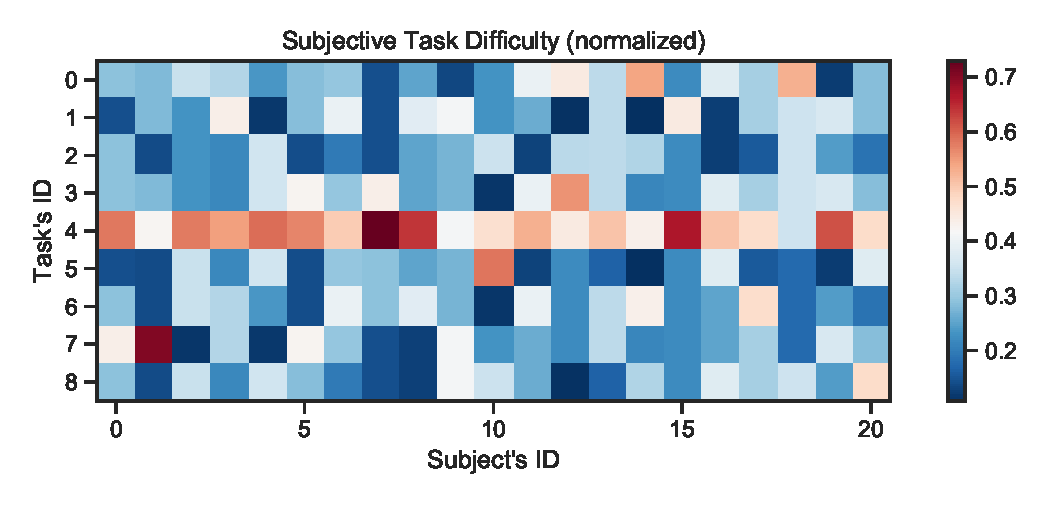
\includegraphics[width=0.8\textwidth]{figures/difficulty}
    \caption{Subjective difficulty score: each column indicates an individual subject and
    each row indicates a browsing task. Tasks from 0 to 8 represent Amazon Goal Oriented Task,
    Amazon Fuzzy Task, Amazon Exploring Task; Medium Goal Oriented Task, Medium Fuzzy Task,
    Medium Exploring Task, Dribbble Goal Oriented Task, Dribbble Fuzzy Task and Dribbble Exploring Task
    respectively.
    From this heat map, we clearly observes Medium Fuzzy Task is the most difficulty task
    according to the subjects voted subjective difficulty, a significant test confirmed this observation.}
    \label{fig:difficulty}
\end{figure}

To generalize the task difficulty, the null hypothesis ($H_0$): the difficulty of fuzzy task is not greater
than exploring task and alternative hypothesis ($H_1$): the difficulty of fuzzy task is greater than
exploring task. We conduct non-parametric one-tailed Kolmogorov-Smirnov test
\cite{massey1951kolmogorov}, under null hypothesis, $p=2.54\times 10^{-5} < 0.05$, reject $H_0$.
Similarly, we compare difficulty score on goal oriented task and exploring task (with corresponding hypothesis, 
$p=0.00534 < 0.05$), difficulty score on fuzzy task and goal oriented task (with corresponding hypothesis, 
$p=0.0145 < 0.05$), all rejects $H_0$. Therefore we concludes the task difficulty is ordered
as follows: \emph{difficulty of fuzzy task $>$ difficulty of goal oriented task $>$ difficulty of exploring task.}

\subsubsection{t-SNE}

\subsubsection{Prediction Accuracy}

\subsubsection{F1}


\subsection{Rationality of Designed Tasks}


\subsection{Explored Model Architecture Comparasion}

\subsection{Action Path Visualization}


\subsection{Discussion}

% 分析实验结果,对比的实验结果包括:

%  任务本身的分析,对任务的难度进行讨论

\cleardoublepage